\documentclass[%
    paper=A4,                   % paper size --> A4 is default in Germany
    twoside=true,               % onesite or twoside printing
    openright,                  % doublepage cleaning ends up right side
    parskip=full,               % spacing value / method for paragraphs
    chapterprefix=true,         % prefix for chapter marks
    11pt,                       % font size
    headings=normal,            % size of headings
    bibliography=totoc,         % include bib in toc
    listof=totoc,               % include listof entries in toc
    titlepage=on,               % own page for each title page
    captions=tableabove,        % display table captions above the float env
    draft=true,                 % value for draft version
]{scrreprt}%

\usepackage[utf8]{inputenc}
\usepackage[english]{babel}
\usepackage[%
    figuresep=colon,%
    sansserif=false,%
    hangfigurecaption=false,%
    hangsection=true,%
    hangsubsection=true,%
    colorize=full,%
    colortheme=bluemagenta,%
    bibsys=bibtex,%
    bibfile=references,%
    bibstyle=alphabetic,%
]{cleanthesis}
\usepackage{subfiles}
\usepackage{amsmath}
\usepackage{amssymb}
\usepackage[inference]{semantic}
\usepackage{galois}
\usepackage{algpseudocode}
\usepackage{graphicx}
\usepackage{url}
\usepackage{IEEEtrantools}

%\listfiles  % Debug LaTeX Information

\newcommand{\thesisTitle}{Structural Optimization of Numerical Programs}
\newcommand{\thesisName}{Xitong Gao}
\newcommand{\thesisDate}{\today}
\newcommand{\thesisVersion}{0.0.1}

\newcommand{\thesisFirstSupervisor}{George A. Constantinides}
% \newcommand{\thesisSecondSupervisor}{John Smith}

\newcommand{\thesisUniversity}{\protect{Imperial College London}}
\newcommand{\thesisUniversityDepartment}{%
    Department of Electrical and Electronic Engineering}
% \newcommand{\thesisUniversityInstitute}{Institut for Clean Thesis Dev}
\newcommand{\thesisUniversityGroup}{Circuits and Systems Research Group}
\newcommand{\thesisUniversityCity}{London}
\newcommand{\thesisUniversityStreetAddress}{South Kensington Campus}
\newcommand{\thesisUniversityPostalCode}{SW7 2AZ}

\hypersetup{%
    pdftitle={\thesisTitle},    %   - title (PDF meta)
    pdfauthor={\thesisName},    %   - author (PDF meta)
    plainpages=false,           %   -
    colorlinks=false,           %   - colorize links?
    pdfborder={0 0 0},          %   -
    breaklinks=true,            %   - allow line break inside links
    bookmarksnumbered=true,     %
    bookmarksopen=true          %
}

\newcommand{\todo}[1]{\{\{\textbf{TODO:} {#1}\}\}\typeout{TODO: {#1}}}

\newcommand{\eg}{\textit{e.g.}}
\newcommand{\etc}{\textit{etc.}}
\newcommand{\etal}{\textit{et~al.}}
\newcommand{\ie}{\textit{i.e.}}

\DeclareMathOperator{\roundup}{\uparrow^\sharp_\circ}
\DeclareMathOperator{\rounddown}{\downarrow^\sharp_\circ}
\DeclareMathOperator{\fresh}{\mathit{fresh}}
\DeclareMathOperator{\eqstep}{\blacktriangleright}
\DeclareMathOperator{\dom}{\mathrm{Dom}}
\DeclareMathOperator{\area}{\mathrm{Area}}
\DeclareMathOperator{\error}{\mathrm{Error}}
\DeclareMathOperator{\abserr}{\mathrm{AbsError}}
\DeclareMathOperator{\abs}{\mathrm{abs}}
\DeclareMathOperator{\frontier}{\textsc{Frontier}}

\newcommand{\naturalset}{\ensuremath\mathbb{N}}
\newcommand{\realset}{\ensuremath\mathbb{R}}
\newcommand{\floatset}{\ensuremath\mathbb{F}}
\newcommand{\powersetof}[1]{\ensuremath\mathcal{P}\left({#1}\right)}
\newcommand{\intervalset}{\ensuremath\mathbf{Interval}}
\newcommand{\floatintervalset}{\ensuremath\intervalset_\floatset}
\newcommand{\errorset}{\ensuremath\mathbb{E}^\sharp}
\newcommand{\labelset}{\ensuremath\mathbf{Label}}
\newcommand{\exprset}{\ensuremath\mathbf{Expr}}
\newcommand{\varset}{\ensuremath\mathbf{Var}}
\newcommand{\env}[1]{\ensuremath\mathbf{Env}_{#1}}
\newcommand{\eqrel}{\ensuremath\mathbin{\rhd}}
\newcommand{\enter}[1]{\ensuremath{A({#1})}}
\newcommand{\interval}[2]{\ensuremath\left[{#1}, {#2}\right]}
\newcommand{\lattice}[2]{\ensuremath\left<{#1}, {#2}\right>}
\newcommand{\join}{\ensuremath\sqcup}
\newcommand{\meet}{\ensuremath\sqcap}

\newcommand{\marteltrace}{\texttt{martel\_trace}}
\newcommand{\frontiertrace}{\texttt{frontier\_trace}}
\newcommand{\greedytrace}{\texttt{greedy\_trace}}

\begin{document}

% Front matter
\pagenumbering{roman}           % roman page numbing (invisible for empty page style)
\pagestyle{empty}               % no header or footers
% !TEX root = ../thesis-example.tex
%
% ------------------------------------  --> cover title page
\begin{titlepage}
	\pdfbookmark[0]{Cover}{Cover}
	\flushright
	\hfill
	\vfill
	{\LARGE\thesisTitle \par}
	\rule[5pt]{\textwidth}{.4pt} \par
	{\Large\thesisName}
	\vfill
	\textit{\large\thesisDate} \\
	Version: \thesisVersion
\end{titlepage}


% ------------------------------------  --> main title page
\begin{titlepage}
	\pdfbookmark[0]{Titlepage}{Titlepage}
	\tgherosfont
	\centering

	
\includegraphics[width=6cm]{imperial_logo} \\[4mm]
    % {\Large \thesisUniversity} \\[4mm]
	\textsf{\thesisUniversityDepartment} \\
	% \textsf{\thesisUniversityInstitute} \\
	\textsf{\thesisUniversityGroup} \\

	\vfill
	{\LARGE \color{ctcolortitle}\textbf{\thesisTitle} \\[10mm]}
	{\Large \thesisName} \\

	\vfill
	% \begin{minipage}[t]{.27\textwidth}
		% \raggedleft
		% \textit{1. Reviewer}
	% \end{minipage}
	% \hspace*{15pt}
	% \begin{minipage}[t]{.65\textwidth}
		% {\Large \thesisFirstReviewer} \\
		  % {\small \thesisFirstReviewerDepartment} \\[-1mm]
		% {\small \thesisFirstReviewerUniversity}
	% \end{minipage} \\[5mm]
	% \begin{minipage}[t]{.27\textwidth}
		% \raggedleft
		% \textit{2. Reviewer}
	% \end{minipage}
	% \hspace*{15pt}
	% \begin{minipage}[t]{.65\textwidth}
		% {\Large \thesisSecondReviewer} \\
		  % {\small \thesisSecondReviewerDepartment} \\[-1mm]
		% {\small \thesisSecondReviewerUniversity}
	% \end{minipage} \\[10mm]
	\begin{minipage}[t]{.27\textwidth}
		\raggedleft
		\textit{Supervisor}
	\end{minipage}
	\hspace*{15pt}
	\begin{minipage}[t]{.65\textwidth}
		\thesisFirstSupervisor%\ and \thesisSecondSupervisor
	\end{minipage} \\[10mm]
    \begin{minipage}[t]{.8\textwidth}
        {\small
            Submitted in part fulfilment of the requirements for the degree of
            Doctor of Philosophy of Imperial College London and the Diploma of
            Imperial College London
        }
    \end{minipage} \\[10mm]

	\thesisDate \\

\end{titlepage}


% ------------------------------------  --> lower title back for single page layout
\hfill
\vfill
{
	\small
	\textbf{\thesisName} \\
	\textit{\thesisTitle} \\
	\thesisDate \\
	% Reviewers: \thesisFirstReviewer\ and \thesisSecondReviewer \\
	Supervisor: \thesisFirstSupervisor%\ and \thesisSecondSupervisor
	\\[1.5em]
    \textbf{\thesisUniversity} \\
	\textit{\thesisUniversityGroup} \\
	% \thesisUniversityInstitute \\
	\thesisUniversityDepartment \\
	\thesisUniversityStreetAddress \\
	\thesisUniversityPostalCode\ and \thesisUniversityCity
}
                   % INCLUDE: all titlepages
\cleardoublepage

\pagestyle{plain}               % display just page numbers
\pdfbookmark[0]{Abstract}{Abstract}
\chapter*{Abstract}
\label{sec:abstract}
\vspace*{-10mm}

This thesis introduces a new technique, and its associated tool \soap, to
automatically perform source-to-source optimization of numerical programs,
specifically targeting the trade-off among numerical accuracy, latency, and
resource usage as a \acrlong{hls} flow for \acrshort{fpga} implementations.  A
new intermediate representation, \acrshort{mir}, is introduced to carry out
the abstraction and optimization of numerical programs.  Equivalent structures
in \acrshortpl{mir} are efficiently discovered using methods based on formal
semantics by taking into account axiomatic rules from real arithmetic, such as
associativity, distributivity and others, in tandem with program equivalence
rules that enable control-flow restructuring and eliminate redundant array
accesses.  For the first time, we bring rigorous approaches from software
static analysis, specifically formal semantics and \acrlong{ai}, to bear
on program transformation for \acrlong{hls}.  New abstract semantics are
developed to generate a computable subset of equivalent \acrshortpl{mir}
from an original \acrshort{mir}.  Using formal semantics, three objectives
are calculated for each \acrshort{mir} representing a pipelined numerical
program: the accuracy of computation and an estimate of resource utilization
in \acrshort{fpga} and the latency of program execution.  The optimization of
these objectives produces a Pareto frontier consisting of a set of equivalent
\acrshortpl{mir}.  We thus go beyond existing literature by not only optimizing
the precision requirements of an implementation, but changing the structure
of the implementation itself.  Using \soap{} to optimize the structure of a
variety of real world and artificially generated arithmetic expressions in
single precision, we improve either their accuracy or the resource utilization
by up to 60\%.  When applied to a suite of computational intensive numerical
programs from PolyBench and Livermore Loops benchmarks, \soap{} has generated
circuits that enjoy up to a 12$\times$ speedup, with a simultaneous 7$\times$
increase in accuracy, at a cost of up to 4$\times$ more \acrshortpl{lut}.
                % INCLUDE: the abstracts (english and german)
\cleardoublepage

% !TEX root = ../thesis-example.tex
%
\pdfbookmark[0]{Acknowledgement}{Acknowledgement}
\chapter*{Acknowledgement}
\label{sec:acknowledgement}
\vspace*{-10mm}

\todo{Acknowledgement goes here\textellipsis}
         % INCLUDE: acknowledgement
\cleardoublepage

\setcounter{tocdepth}{2}        % define depth of toc
\tableofcontents                % display table of contents
\cleardoublepage

% Body matter
\pagenumbering{arabic}          % arabic page numbering
\setcounter{page}{1}            % set page counter
\pagestyle{maincontentstyle}    % fancy header and footer

\doublespacing

% Main text
\chapter{Introduction}

\chapter{Background}

\chapter{Structural Optimization of Arithmetic Expressions}
\label{chp:stropt}

% \begin{abstract}
    % This paper introduces SOAP, a new tool to automatically optimize the
% structure of arithmetic expressions for FPGA implementation as part of a
% high level synthesis flow, taking into account axiomatic rules derived
% from real arithmetic, such as distributivity, associativity and others. We
% explicitly target an optimized area/accuracy trade-off, allowing arithmetic
% expressions to be automatically re-written for this purpose. For the first
% time, we bring rigorous approaches from software static analysis, specifically
% formal semantics and abstract interpretation, to bear on source-to-source
% transformation for high-level synthesis. New abstract semantics are developed
% to generate a computable subset of equivalent expressions from an original
% expression. Using formal semantics, we calculate two objectives, the accuracy
% of computation and an estimate of resource utilization in FPGA\@. The
% optimization of these objectives produces a Pareto frontier consisting of a
% set of expressions. This gives the synthesis tool the flexibility to choose
% an implementation satisfying constraints on both accuracy and resource
% usage. We thus go beyond existing literature by not only optimizing the
% precision requirements of an implementation, but changing the structure of the
% implementation itself. Using our tool to optimize the structure of a variety of
% real world and artificially generated examples in single precision, we improve
% either their accuracy or the resource utilization by up to 60\%.
% \end{abstract}

\section{Introduction}

Our previous chapter introduced a new methodology to efficiently restructure
arithmetic expressions for the optimized trade-off between two performance
metrics, \ie~numerical accuracy when evaluated and area usage in synthesized
FPGA implementations.  However, this method has a substantial limitation when
applied to general numerical programs, that is, it can only be applied to
straight-line codes without control structures such as branches and loops.

The structural optimization of general numerical programs is much more complex
than that of arithmetic expressions.  The reasons are two-fold.  First,
during program execution, variables are often updated with new values.  Our
optimization should therefore perform static analysis on the values of
variables, and use the result to optimize specifically for the trade-off
between accuracy and resource usage.  Second, it is much more difficult to
formally define program equivalence, and subsequently, to search efficiently
for optimized equivalent programs.  For instance, even without the introduction
of branches and loops, the following two programs are equivalent, but
syntactically, they are very different.  In practice, it is desirable to
eliminate as much as possible the need for these syntactic rewrites that do not
affect our performance metrics.

\begin{figure}[ht]
    \centering
    \subfloat[$P_1$]{%
        \shortstack[l]{%
            \texttt{x = x + 1;} \\
            \texttt{y = 2 * x;} \\
            \texttt{x = x + 3;}
        }
    } \qquad \qquad
    \subfloat[$P_2$]{%
        \shortstack[l]{%
            \texttt{y = x + 1;} \\
            \texttt{x = y;} \\
            \texttt{y = y * 2;} \\
            \texttt{x = x + 3;}
        }
    }
    \caption{Two programs that are equivalent but syntactically different.}
    \label{fig:equiv_progs}
\end{figure}

Therefore, in this chapter, we provide answers to these two above issues.  In
the meantime, we propose a new general \emph{program} optimization technique
for numerical algorithms, which allows \texttt{if} statements as well as
\texttt{while} loops, and developed its accompanied tool, \newsoap, to enable
the joint optimization of accuracy and resource usage, as well as the trade-off
between these performance metrics.  We develop a tool, which we call \newsoap,
to perform source-to-source optimization of numerical programs targeting FPGAs,
and generate implementations that trade off resource usage and numerical
accuracy.

% floating-point arithmetic has round-off errors, exploit equivalence

Similar to the approach we have proposed in Chapter~\ref{chp:stropt}, we
exploit equivalence rules such as such as \emph{associativity} $(a + b) +
c \equiv a + (b + c)$, and \emph{distributivity} $(a + b) \times c \equiv
a \times c + b \times c$ to automatically optimize implementations for
the optimal trade-off between resource usage, \ie~the number of LUTs and
DSP elements utilized, and accuracy when evaluated using floating-point
computations.  For example, with single precision floating-point format, our
tool found that give an input $x \in [0, 100]$ and $y \in [0, 2]$, then the
program:
\begin{lstlisting}
    if (x < 1) {
        x = (x + y) + 0.1;
    } else {
        x = x + (y + 0.1);
    }
\end{lstlisting}
is most accurate when rewritten in the following form:
\begin{lstlisting}
    if (x < 1) {
        x = (x + 0.1) + y;
    } else {
        x = x + (y + 0.1);
    }
\end{lstlisting}
On the other hand, the original program uses fewest resources when
subexpressions are shared and the \iflit~statement is eliminated:
\begin{lstlisting}
    x = x + (y + 0.1);
\end{lstlisting}

This kind of optimization generates a Pareto optimal set of implementations,
which trades off accuracy and area.  A na{\"\i}ve strategy to search for
the Pareto optimal implementations is to discover all possible equivalent
expressions.  However, this would result in combinatorial explosion and become
intractable even for very small expressions~\cite{ioualalen,mouilleron}.  To
remedy this, in Chapter~\ref{chp:stropt} we proposed a novel approach, known
as \soap, to significantly reduce the space and time complexity to produce a
subset of the Pareto frontier.

% program transformation why?

Our program optimization flow is \emph{safe}, \emph{semantics-directed} and
\emph{flexible}. \emph{Safety} means that because we make use of formal
mathematics to optimize programs, our approach can be proved correct, in
the sense that when executed using exact real arithmetic, the transformed
version produces exactly the same output values as the original program.
\emph{Semantics-directed} transformation means that not only do we use
program syntax, but also the semantics to guide optimization and guarantee
safety properties of the optimized program.  Our technique obtains when
necessary, by analyzing the program, a bound and a round-off error bound on
each variable in every program location.  These information are then used
to guide program optimization.  By analyzing and manipulating not only the
syntax, but also the semantics of programs.  The meaning of a \emph{flexible}
program transformation is three-fold.  First, arithmetic computations can be
optimized across assignments, \iflit~statements and \whilelit~loops.  Secondly,
we automatically explore the numerical implications of partial loop unrolling
and loop splitting, which can create more opportunity for minimizing round-off
errors, hence further increases range of options in the Pareto frontier of
trade-offs.  Finally, our method naturally subsumes constant propagation,
redundant code elimination, and also branch and loop fusions.

% Our tool fits in the familiar setting of the high-level synthesis tool flow, as a front-end that performs the source-to-source optimization of

Our main contributions in this chapter are as follows:
\begin{enumerate}
    \vspace{-6pt}
    \item
        A new intermediate representation of the behaviour of numerical
        programs, its structure is designed to be manipulated and analyzed
        with ease.  A new framework of numerical program transformations is
        developed to enable the back and forth translation between the program
        and a new intermediate representation (IR), which preserves the
        semantics of the original program.
    \vspace{-6pt}
    \item
        Semantics-based analyses that reason about not only the resource
        utilization (number of LUTs and DSP elements), and safe ranges of
        values and errors for programs, but also potential errors such as
        overflows and non-termination.
    \vspace{-6pt}
    \item
        A new tool, \newsoap, which trades off resource usage and accuracy
        by providing a safe, semantics-directed and flexible optimization
        targeting numerical programs for high-level synthesis.
    \vspace{-6pt}
\end{enumerate}

Section~\ref{sec:related_work} provides an overview of the existing work
related in both the software and high-level synthesis community.  We then
proceed to define our program syntax in Section~\ref{sec:syntax_definition}.
Using the syntax definition, we provide a detailed formal explanation
of our numerical program transformation, which consists of three
stages.  Section~\ref{sec:program_to_mir}, {}~\ref{sec:transformations},
{}~\ref{sec:code_generation} describe in sequence how numerical programs
can be translated into MIRs, how we infer bounds and error bounds on
variables and analyze resource usage estimates for the efficient discovery
of equivalent structures in the analyzed MIR, and finally, we explain how
a chosen MIR can be translated into an optimized numerical program.  Then
we present the optimization results in Section~\ref{sec:results} and
Section~\ref{sec:conclusion} concludes this chapter.

\section{Related Work}
\label{sec:related_work}

Our work conducts program transformations on our MIR intermediate
representation introduced in Chapter~\ref{chp:progopt}. Alternative program
representations include \emph{static} and \emph{dynamic single assignment
forms} (SSA, DSA)~\cite{rau92, cytron91}, and \emph{control and data flow
graphs} (CDFG)~\cite{gajski94}. These representations are less suitable for
our work because they are all statement-based and do not identify as many
equivalent programs as MIRs do. Dependence graphs~\cite{rau94}, on the other
hand, are designed for the purpose of capturing data flow dependences in
polyhedral methods, but they generally do not preserve enough information for
us to reconstruct a program from the graph itself.

Several HLS tools exploit dependence graph restructuring to improve loop
parallelism, which allows for a smaller initiation interval, and in turn faster
programs.  Tree height reduction~\cite{nicolau91} aims to balance an arithmetic
expression tree using associativity and distributivity. Xilinx's Vivado HLS has
a similar feature called \emph{expression balancing}~\cite{vivado_hls}.  Both
of these methods do not produce optimal loop pipelining, as they do not examine
the implications of loop-carried dependences.  Canis \etal~\cite{canis14}
propose a similar approach called \emph{recurrence minimization}. They
specifically tackle loop pipelining by incrementally restructuring dependence
graphs to minimize longest paths of recurrences. Their method is subsequently
incorporated in LegUp~\cite{legup}, an open-source academic HLS tool.  However,
both LegUp and Vivado HLS only apply associativity in their restructuring.

Most importantly, none of the above mentioned techniques and tools aim to
minimize, or even analyze, the impact of their transformations on resource
usage and accuracy. In many numerically sensitive programs, small round-off
errors would result in catastrophic inaccurate results. Therefore, HLS tools
generally disable this feature by default for floating-point computations. For
this reason, we have developed our tool to optimize not only program latencies,
but also resource usage and accuracy.

% Several authors have considered program transformations that improve
% accuracy or resource usage. Both Damouche~\etal~\cite{damouche15} and
% Panchekha \etal~\cite{panchekha15} propose methods for optimizing numerical
% accuracy in software using equivalences from real arithmetic, but they
% consider individual expressions only, and have no control structure
% manipulation, such as optimizing across basic blocks or partial loop
% unrolling.  Hosangadi \etal~\cite{hosangadi} minimize resource usage
% by employing symbolic algebra to reduce the number of operations, and
% Peymandoust~\etal~\cite{peymandoust} factorize polynomials using Gr{\"o}bner
% bases; both only deal with polynomial arithmetic expressions. The \SOAP{} tool
% of Gao~\etal~\cite{soap2} simultaneously optimizes numerical programs for
% resource usage and accuracy, but is unable to analyze latency.

%%% Local Variables:
%%% mode: latex
%%% TeX-master: "paper"
%%% End:

\section{Abstract Interpretation}
\label{bg:sec:abstract_interpretation}

This section starts by introducing the basic concepts of program semantics
and the abstract interpretation framework, a static analysis technique.  This
is then extended to define a scalable analysis capturing accuracy.  Later in
Chapter~\ref{chp:progopt} we accommodate sequential statements, \iflit~branches
and \whilelit~loops in the accuracy analysis, and in Chapter~\ref{chp:latopt},
we further improve our analysis by supporting multi-dimensional arrays.


\subsection{Intervals}
\label{bg:sub:intervals}

We illustrate these concepts by putting the familiar idea of \emph{interval
arithmetic}~\cite{moore} in the framework of abstract interpretation. As
an illustration, consider the following expression and its DFG in
Figure~\ref{bg:fig:sample_tree}\@:
\begin{equation}
    (a + b) \times (a + b)
    \label{bg:eq:absint_sample}
\end{equation}
\begin{figure}[ht]
    \centering
    \includegraphics[scale=0.6]{sample_tree}
    \caption{The DFG for the sample expression.}\label{bg:fig:sample_tree}
\end{figure}

We may wish to ask: if initially $a$ and $b$ are real numbers in the range of
$[0.2, 0.3]$ and $[2, 3]$ respectively, what would be the outcome of evaluating
this expression with real arithmetic? A straightforward approach is simulation.
Evaluating the expression for a large quantity of inputs will produce a set
of possible outputs of the expression. However the simulation approach is
unsafe, since there are infinite number of real-valued inputs possible and it
is infeasible to simulate for all.

A better method might be to represent the possible values of $a$ and $b$ using
ranges. To compute the ranges of its output values, we could operate on ranges
rather than values (note that the superscript $\sharp$ denotes ranges). Assume
that $a^\sharp_{init} = [0.2, 0.3]$, $b^\sharp_{init} = [2, 3]$, which are the
input ranges of $a$ and $b$, and $\enter{l}$ where $l \in \{1, 2, 3, 4\}$ are
the intervals of the outputs of the boxes labelled with $l$ in the DFG\@. We
extract the data flow from the DFG to produce the following set of equations:
\begin{equation}
    \begin{aligned}
        \enter{1} &= a^\sharp_{init} \\
        \enter{2} &= b^\sharp_{init} \\
        \enter{3} &= \enter{1} + \enter{2} \\
        \enter{4} &= \enter{3} \times \enter{3}
    \end{aligned}
    \label{bg:eq:absint_sample_analysis}
\end{equation}
For the equations above to make sense, addition and multiplication need to be
defined on intervals. We may define the following interval operations:
\begin{equation}
    \begin{aligned}
        \interval{a}{b} + \interval{c}{d} &= \interval{a + c}{b + d} \\
        \interval{a}{b} - \interval{c}{d} &=  \interval{a - d}{b - c} \\
        \interval{a}{b} \times \interval{c}{d} &=
            \interval{\min(s)}{\max(s)} \\
        \text{where~} s &= \{ a \times c, a \times d, b \times c, b \times d \}
    \end{aligned}
    \label{bg:eq:interval_operations}
\end{equation}
The solution to the set of~\eqref{bg:eq:absint_sample_analysis} for $\enter{4}$
is $[4.84, 10.89]$, which represents a safe bound on the output at the end
of program execution. Note that in actual execution of the program, the
semantics represent the values of intermediate variables, which are real
values. In our case, a set of real values forms the set of all possible
values produced by our code. However computing this set precisely is not,
in general, a possible task. Instead, we use abstract interpretation based
on intervals, which gives the abstract semantics of this program. Here, we
have achieved a classical interval analysis by \emph{defining} the meaning of
addition and multiplication on abstract mathematical structures (in this case
intervals) which capture a safe approximation of the original semantics of the
program.

Later in Sections~\ref{so:sec:resource}~and~\ref{so:sec:equivalent} of
Chapter~\ref{chp:stropt}, we further generalize the idea by defining the
meaning of these operations on more complex abstract structures which allow
us to scalably reason about the area of FPGA implementations and equivalent
program structures respectively.


\subsection{Accuracy Analysis}
\label{bg:sub:accuracy}

Because we optimize numerical programs in a way that may have significant
impact on accuracy, and one of our objectives is to minimize round-off error
in the process, it is necessary to perform accuracy analysis on optimized
candidates.

Since our numerical programs make use of floating-point arithmetic, we first
introduce the concepts of the floating-point representation~\cite{ieee754}. Any
values $v$ representable in floating-point with standard exponent offset can be
expressed with the format given by the following equation:
\begin{equation}
    v = s \times 2^{e + 2^{k - 1} - 1} \times 1.{m_1 m_2 m_3 \ldots m_p}
    \label{bg:eq:floating_point}
\end{equation}
In~\eqref{bg:eq:floating_point}, the bit $s$ is the sign bit, the $k$-bit
unsigned integer $e$ is known as the exponent bits, and the $p$-bits $m_1 m_2
m_3 \ldots m_p$ are the mantissa bits, here we use $1.{m_1 m_2 m_3 \ldots m_p}$
to indicate a fixed-point number represented in unsigned binary format.

Because of the finite characteristic of IEEE 754 floating-point format, it
is not always possible to represent exact values with it. Computations in
floating-point arithmetic often induces roundoff errors. Therefore, following
Martel~\cite{martel07}, we bound with ranges the values of floating-point
calculations, as well as their roundoff errors. Our accuracy analysis
determines the bounds of all possible outputs and their associated range of
roundoff errors for expressions. For example, assume that real variables $a
\in [0.2, 0.3]$, $b \in [2.3, 2.4]$, it is possible to derive that in single
precision floating-point computation with rounding to the nearest, ${(a + b)}^2
\in [6.24999857, 7.29000187]$ and the error caused by this computation is
bounded by $[-1.60634534\times10^{-6}, 1.60634534\times10^{-6}]$.

We employ abstract error semantics for the calculation of errors described
in~\cite{ioualalen, martel07}. First we define the domain $\errorset
= \floatintervalset\times\intervalset$, where $\intervalset$ and
$\floatintervalset$ respectively represent the set of real intervals, and
the set of floating-point intervals (intervals exactly representable in
floating-point arithmetic). The value $(x^\sharp, \mu^\sharp) \in \errorset$
represents a safe bound on floating-point values and the accumulated error
represented as a range of real values. Then addition and multiplication can be
defined for the semantics as in~\eqref{bg:eq:error_semantics}:
\begin{equation}
    \begin{aligned}
        \left( x^\sharp_1, \mu^\sharp_1 \right) +
        \left( x^\sharp_2, \mu^\sharp_2 \right)
    &=  \left(
            \roundup{x^\sharp_1 + x^\sharp_2},
            \mu^\sharp_1 + \mu^\sharp_2 +
            \rounddown{x^\sharp_1 + x^\sharp_2}
        \right) \\
        \left( x^\sharp_1, \mu^\sharp_1 \right) -
        \left( x^\sharp_2, \mu^\sharp_2 \right)
    &=  \left(
            \roundup{x^\sharp_1 - x^\sharp_2},
            \mu^\sharp_1 - \mu^\sharp_2 +
            \rounddown{x^\sharp_1 - x^\sharp_2}
        \right) \\
        \left( x^\sharp_1, \mu^\sharp_1 \right) \times
        \left( x^\sharp_2, \mu^\sharp_2 \right)
    &=  \left(
            \roundup{x^\sharp_1 \times x^\sharp_2},
            x^\sharp_1 \times \mu^\sharp_2 + x^\sharp_2 \times \mu^\sharp_1 +
            \mu^\sharp_1 \times \mu^\sharp_2 +
            \rounddown{x^\sharp_1 \times x^\sharp_2}
        \right) \\
    &\qquad\qquad\qquad\qquad\qquad\qquad\text{~for~}
        \left( x^\sharp_1, \mu^\sharp_1 \right) \in \errorset,
        \left( x^\sharp_2, \mu^\sharp_2 \right) \in \errorset
    \end{aligned}
    \label{bg:eq:error_semantics}
\end{equation}

The addition, subtraction and multiplication of intervals follow
the standard rules of interval arithmetic defined earlier
in~\eqref{bg:eq:interval_operations}.  In~\eqref{bg:eq:error_semantics}, the
function $\rounddownop: \intervalset \to \intervalset$ determines the range
of roundoff error due to the floating-point computation under one of the
\emph{rounding modes} $\circ \in \{ -\infty, \infty, 0, \neg0, \sim \}$ which
are round towards negative infinity, towards infinity, towards zero, away from
zero and towards nearest floating-point value respectively. It is defined as:
\begin{equation}
    \begin{aligned}
        & \downarrow^\sharp_\circ([a, b]) = \left\{
            \begin{aligned}
                & \left[ -\frac{z}{2}, \frac{z}{2}\right]
                    & \quad \circ & \text{~is~}\sim \\
                & \left[ -z, z\right]
                    & \quad \circ & \in \{ -\infty, \infty, 0, \neg0 \}
            \end{aligned}
        \right. \\
        & \qquad\qquad\qquad\qquad \text{where~} z = \max(ulp(a), ulp(b))
    \end{aligned}
\end{equation}
Here $z$ denotes the maximum rounding error that can occur for values
within the range $[a, b]$, and the unit of the last place (ulp) function
$ulp(x)$~\cite{muller} characterizes the distance between two adjacent
floating-point values $f_1$ and $f_2$ satisfying $f_1 \leq x \leq
f_2$~\cite{goldberg}. In our analysis, the function $ulp$ is defined as:
\begin{equation}
    ulp(x) = 2^{e(x) + 2^{k - 1} - 1} \times 2^{-p}
\end{equation}
where $e(x)$ is the exponent of $x$, $k$ and $p$ are the parameters of the
floating-point format as defined in~\eqref{bg:eq:floating_point}. The function
$\roundupop: \intervalset \to \floatintervalset$ computes the floating-point
bound from a real bound, by rounding the infimum $a$ and supremum $b$ of the
input interval $[a, b]$:
\begin{equation}
    \roundupop\left(\left[a, b\right]\right)
    = {\left[
        \uparrow_\circ{\left(a\right)},
        \uparrow_\circ{\left(b\right)}
    \right]}_\floatset
\end{equation}
where the subscript $\floatset$ indicates the interval is a floating-point
interval, and we define $\uparrow_\circ: \realset \to \floatset$ to be the
function that rounds a real number to a floating-point value, under the
rounding mode $\circ$.

Expressions can be evaluated for their accuracy by the method as follows.
Initially the expression is parsed into a data flow graph (DFG). By way of
illustration, the sample expression ${(a + b)}^2$ has the tree structure
in Figure~\ref{bg:fig:sample_tree}. Then the exact ranges of values of $a$ and
$b$ are converted into the abstract semantics using a cast operation as in
\eqref{bg:eq:cast}:
\begin{equation}
    \mathrm{cast}\left(x^\sharp\right) = \left(
        \roundup{x^\sharp}, \rounddown{x^\sharp}
    \right)
    \label{bg:eq:cast}
\end{equation}
For example, for the real variable $a \in [0.2, 0.3]$ under single precision
with rounding to nearest,
\begin{equation}
    \mathrm{cast}\left([0.2, 0.3]\right) = \left(
        {\left[0.200000003, 0.300000012\right]}_\floatset,
        \left[-1/67108864, 1/67108864\right]
    \right)
\end{equation}
After this, the propagation of bounds in the data flow graph is carried out as
described in Section~\ref{bg:sub:intervals}, where the difference is the abstract
error semantics defined in~\eqref{bg:eq:error_semantics} is used in lieu of the
interval semantics. At the root of the tree (\ie~the exit of the DFG) we find
the value of the accuracy analysis result for the expression.

\section{Novel Semantics}
\label{sec:semantics}

\subsection{Accuracy Analysis}

We first introduce the concepts of the floating-point
representation~\cite{ieee754}. Any values $v$ representable in floating-point
with standard exponent offset can be expressed with the format given by the
following equation:
\begin{equation}
    v = s \times 2^{e + 2^{k - 1} - 1} \times 1.{m_1 m_2 m_3 \ldots m_p}
    \label{eq:floating_point}
\end{equation}
In~\eqref{eq:floating_point}, the bit $s$ is the sign bit, the $k$-bit unsigned
integer $e$ is known as the exponent bits, and the $p$-bits $m_1 m_2 m_3
\ldots m_p$ are the mantissa bits, here we use $1.{m_1 m_2 m_3 \ldots m_p}$ to
indicate a fixed-point number represented in unsigned binary format.

Because of the finite characteristic of IEEE 754 floating-point format, it
is not always possible to represent exact values with it. Computations in
floating-point arithmetic often induces roundoff errors. Therefore, following
Martel~\cite{martel07}, we bound with ranges the values of floating-point
calculations, as well as their roundoff errors. Our accuracy analysis
determines the bounds of all possible outputs and their associated range
of roundoff errors for expressions. For example, assume that $a \in [0.2,
0.3]$, $b \in [2.3, 2.4]$, it is possible to derive that in single precision
floating-point computation with rounding to the nearest, ${(a + b)}^2 \in
[6.24999857, 7.29000187]$ and the error caused by this computation is bounded
by $[-1.60634534\times10^{-6}, 1.60634534\times10^{-6}]$.

We employ abstract error semantics for the calculation of errors described
in~\cite{ioualalen, martel07}. First we define the domain $\errorset
= \floatintervalset\times\intervalset$, where $\intervalset$ and
$\floatintervalset$ respectively represent the set of real intervals, and
the set of floating-point intervals (intervals exactly representable in
floating-point arithmetic). The value $(x^\sharp, \mu^\sharp) \in \errorset$
represents a safe bound on floating-point values and the accumulated error
represented as a range of real values. Then addition and multiplication can be
defined for the semantics as in~\eqref{eq:error_semantics}:
\begin{equation}
    \begin{aligned}
        (x^\sharp_1, \mu^\sharp_1) + (x^\sharp_2, \mu^\sharp_2)
    &=  (\roundup{x^\sharp_1 + x^\sharp_2},
         \mu^\sharp_1 + \mu^\sharp_2 +
         \rounddown{x^\sharp_1 + x^\sharp_2}) \\
        (x^\sharp_1, \mu^\sharp_1) - (x^\sharp_2, \mu^\sharp_2)
    &=  (\roundup{x^\sharp_1 - x^\sharp_2},
         \mu^\sharp_1 - \mu^\sharp_2 +
         \rounddown{x^\sharp_1 - x^\sharp_2}) \\
        (x^\sharp_1, \mu^\sharp_1) \times (x^\sharp_2, \mu^\sharp_2)
    &=  (\roundup{x^\sharp_1 \times x^\sharp_2},
            x^\sharp_1 \times \mu^\sharp_2 + x^\sharp_2 \times \mu^\sharp_1 +
            \mu^\sharp_1 \times \mu^\sharp_2 +
            \rounddown{x^\sharp_1 \times x^\sharp_2}) \\
    &\qquad\qquad\qquad\qquad\qquad\qquad\text{~for~}
        (x^\sharp_1, \mu^\sharp_1) \in \errorset,
        (x^\sharp_2, \mu^\sharp_2) \in \errorset
    \end{aligned}
    \label{eq:error_semantics}
\end{equation}
The addition, subtraction and multiplication of intervals follow the standard
rules of interval arithmetic defined earlier in~\eqref{eq:interval_operations}.
In~\eqref{eq:error_semantics}, the function $\rounddownop: \intervalset \to
\intervalset$ determines the range of roundoff error due to the floating-point
computation under one of the rounding modes $\circ \in \{ -\infty, \infty, 0,
\neg0, \sim \}$ which are round towards negative infinity, towards infinity,
towards zero, away from zero and towards nearest floating-point value
respectively. It is defined as:
\begin{equation}
    \begin{aligned}
        & \downarrow^\sharp_\circ([a, b]) = \left\{
            \begin{aligned}
                & \left[ -\frac{z}{2}, \frac{z}{2}\right]
                    & \quad \circ & \text{~is~}\sim \\
                & \left[ -z, z\right]
                    & \quad \circ & \in \{ -\infty, \infty, 0, \neg0 \}
            \end{aligned}
        \right. \\
        & \qquad\qquad\qquad\qquad \text{where~} z = \max(ulp(a), ulp(b))
    \end{aligned}
\end{equation}
Here $z$ denotes the maximum rounding error that can occur for values
within the range $[a, b]$, and the unit of the last place (ulp) function
$ulp(x)$~\cite{muller} characterizes the distance between two adjacent
floating-point values $f_1$ and $f_2$ satisfying $f_1 \leq x \leq
f_2$~\cite{goldberg}. In our analysis, the function $ulp$ is defined as:
\begin{equation}
    ulp(x) = 2^{e(x) + 2^{k - 1} - 1} \times 2^{-p}
\end{equation}
where $e(x)$ is the exponent of $x$, $k$ and $p$ are the parameters of the
floating-point format as defined in~\eqref{eq:floating_point}. The function
$\roundupop: \intervalset \to \floatintervalset$ computes the floating-point
bound from a real bound, by rounding the infimum $a$ and supremum $b$ of the
input interval $[a, b]$.

Expressions can be evaluated for their accuracy by the method as follows.
Initially the expression is parsed into a data flow graph (DFG). By way of
illustration, the sample expression ${(a + b)}^2$ has the tree structure
in Figure~\ref{fig:sample_tree}. Then the exact ranges of values of $a$ and
$b$ are converted into the abstract semantics using a cast operation as in
\eqref{eq:cast}:
\begin{equation}
    cast(x^\sharp) = (\roundup{x^\sharp}, \rounddown{x^\sharp})
    \label{eq:cast}
\end{equation}
For example, for the variable $a \in [0.2, 0.3]$ under single precision
with rounding to nearest,
\begin{equation}
    cast([0.2, 0.3]) = ([0.200000003, 0.300000012], [-1/67108864, 1/67108864])
\end{equation}
After this, the propagation of bounds in the data flow graph is carried out as
described in Section~\ref{sec:abstract_interpretation}, where the difference is
the abstract error semantics defined in~\eqref{eq:error_semantics} is used in
lieu of the interval semantics. At the root of the tree (\ie~the exit of the
DFG) we find the value of the accuracy analysis result for the expression.

We use the function $\error: \exprset\to\errorset$ throughout this chapter to
represent the analysis of evaluation accuracy, where $\exprset$ denotes the set
of all expressions.

\subsection{Resource Usage Analysis}

Here we define similar formal semantics which calculate an approximation to the
FPGA resource usage of an expression, taking into account common subexpression
elimination. This is important as, for example, rewriting $a \times b + a
\times c$ as $a \times (b + c)$ in the larger expression $(a \times b + a
\times c) + {(a \times b)}^2$ causes the common subexpression $a \times b$ to
be no longer present in both terms. Our analysis must capture this.

The analysis proceeds by labelling subexpressions. Intuitively, the set of
labels $\labelset$, is used to assign unique labels to unique expressions,
so it is possible to easily identify and reuse them. For convenience, let
the function $\fresh: \exprset\to\labelset$ assign a distinct label to each
expression or variable, where $\exprset$ is the set of all expressions. Before
we introduce the labeling semantics, we define the environment $\lambda:
\labelset\to\exprset\cup\{\bot\}$, which is a function that maps labels to
expressions, and $\env{}$ denotes the set of such environments. A label $l$ in
the domain of $\lambda\in\env{}$ that maps to $\bot$ indicates that $l$ does
not map to an expression. An element $(l, \lambda)\in\labelset\times\env{}$
stands for the labeling scheme of an expression. Initially, we map all labels
to $\bot$, then in the mapping $\lambda$, each leaf of an expression is
assigned a unique label, and the unique label $l$ is used to identify the leaf.
That is for the leaf variable or constant $x$:
\begin{equation}
    (l, \lambda) = (\fresh(x), [\fresh(x)\mapsto{x}])
\end{equation}
This equation uses $[\fresh(x)\mapsto{x}]$ to indicate an environment that
maps the label $\fresh(x)$ to the expression $x$ and all other labels map
to $\bot$, in other words, if $l = \fresh(x)$ and $l^\prime \neq l$, then
$\lambda(l) = x$ and $\lambda(l^\prime) = \bot$. For example, for the DFG in
Figure~\ref{fig:sample_tree}, we have for the variables $a$ and $b$:
\begin{equation}
    \begin{aligned}
        (l_a, \lambda_a) &= (\fresh(a), [\fresh(a)\mapsto{a}])
                   = (l_1, [l_1 \mapsto a]) \\
        (l_b, \lambda_b) &= (l_2, [l_2 \mapsto b])
    \end{aligned}
    \label{eq:variable_env}
\end{equation}
Then the environments are propagated in the flow direction of the DFG, using
the following formulation of the labeling semantics:
\begin{equation}
    \begin{aligned}
        (l_x, \lambda_x) \circ (l_y, \lambda_y)
            &= (l, (\lambda_x\odot\lambda_y)
                      [l\mapsto{l_x \circ l_y}]) \\
            \text{where~} l &= \fresh(l_x \circ l_y),
                          \circ\in\{+, -, \times\}
    \end{aligned}
    \label{eq:labeling_semantics}
\end{equation}
Specifically, $\lambda=\lambda_x\odot\lambda_y$ signifies that $\lambda_y$
is used to update the mapping in $\lambda_x$, if the mapping does not
exist in $\lambda_x$, and result in a new environment $\lambda$; and
$\lambda[l\mapsto{x}]$ is a shorthand for $\lambda\odot[l\mapsto{x}]$.
As an example, with the expression in Figure~\ref{fig:sample_tree}, using
\eqref{eq:variable_env}, recall to mind that $l_1 = l_a$, $l_2 = l_b$, we
derive for the subexpression $a + b$:
\begin{equation}
    \begin{aligned}
        (l_{a + b}, \lambda_{a + b})
            &= (l_a, \lambda_a) + (l_b, \lambda_b) \\
            &= (l_3, (\lambda_a \odot \lambda_b) [l_3\mapsto{l_a + l_b}]) \\
            &  \text{where~} l_3 = \fresh(l_a + l_b) \\
            &= (l_3, [l_1\mapsto{a}]\odot
                     [l_2\mapsto{b}]\odot
                     [l_3\mapsto{l_1 + l_2}]) \\
            &= (l_3, [l_1\mapsto{a}, l_2\mapsto{b}, l_3\mapsto{l_1 + l_2}])
    \end{aligned}
\end{equation}
\todo{George: I am a little confused by addition here.  What is the definition
of ``+'' on labels?  If $l_a + l_b$ should be read purely as a syntactic
construct, why does it need a distinct representation as $l_3$?}
Finally, for the full expression $(a + b) \times (a + b)$:
\begin{equation}
    \begin{aligned}
        (l, \lambda)
            &= (l_{a + b}, \lambda_{a + b}) \times
               (l_{a + b}, \lambda_{a + b}) \\
            &= (l_4, [l_1\mapsto{a}, l_2\mapsto{b},
                      l_3\mapsto{l_1 + l_2}, l_4\mapsto{l_3 \times l_3}])
    \end{aligned}
\end{equation}
From the above derivation, it is clear that the semantics capture the reuse
of subexpressions. The estimation of area is performed by counting, for an
expression, the numbers of additions, subtractions and multiplications in
the final labeling environment, then calculating the number of LUTs used to
synthesize the expression. If the number of operators is $n_\circ$ where
$\circ\in\{+,-,\times\}$, then the number of LUTs in total for the expressions
is estimated as $\sum_{\circ\in\{+,-,\times\}} A_\circ n_\circ$, where the
value $A_\circ$ denotes the number of LUTs per $\circ$ operator, which is
dependent on the type of the operator and the floating-point format used to
generate the operator.

In the following sections, we use the function $\area: \exprset\to\naturalset$
to denote our resource usage analysis.

\subsection{Equivalent Expressions Analysis}
\label{sub:equivalent_expressions_analysis}

In earlier sections, we introduce semantics that define additions and
multiplications on intervals, then gradually transition to error semantics that
compute bounds of values and errors, as well as labelling environments that
allow common subexpression elimination, by defining arithmetic operations on
these structures. In this section, we now take the leap from not only analyzing
an expression for its quality, to defining arithmetic operations on sets of
equivalent expressions, and use these rules to discover equivalent expressions.
Before this, it is necessary to formally define equivalent expressions and
functions to discover them.

\subsubsection{Discovering Equivalent Expressions}

From an expression, a set of equivalent expressions can be discovered by our
\emph{equivalence relation} $\eqrel$ on the set of all expressions $\exprset$,
and $\eqrel \subset \exprset\times\exprset$.  It is noteworthy that a relation
is said to be an equivalence relation when it is reflexive, symmetric and
transitive, \ie~for all $e_1, e_2, e_3 \in \exprset$, we have the following
rules in our inference system:
\begin{equation}
    \begin{aligned}
        \text{Reflexivity}
            &: e_1 \eqrel e_1 \\
        \text{Symmetry}
            &: \text{~if~} e_1 \eqrel e_2,
            \text{~then~} e_2 \eqrel e_1 \\
        \text{Transitivity}
            &: \text{~if~} e_1 \eqrel e_2 \text{~and~} e_2 \eqrel e_3,
            \text{~then~} e_1 \eqrel e_3.
    \end{aligned}
\end{equation}

We extend our inference system with additional rules that relate equivalent
expressions.  Let's define $e_1, e_2, e_3 \in \exprset$, $v_1, v_2, v_3 \in
\realset$, and $\circ \in \{+, \times\}$.  First, the arithmetic rules are:
\begin{equation*}
    \begin{aligned}
        \text{Associativity}(\circ)
            &: (e_1 \circ e_2) \circ e_3 \eqrel e_1 \circ (e_2 \circ e_3) \\
        \text{Commutativity}(\circ)
            &: e_1 \circ e_2 \eqrel e_2 \circ e_1 \\
        \text{Distributivity}
            &: e_1 \times (e_2 + e_3) \eqrel e_1 \times e_2 + e_1 \times e_3
    \end{aligned}
\end{equation*}
Secondly, the reduction rules are:
\begin{equation*}
    \begin{aligned}
        \text{Identity}(\times)
            &: e_1 \times 1 \eqrel e_1 \quad &
        \text{ZeroProp}
            &: e_1 \times 0 \eqrel 0 \\
        \text{Identity}(+)
            &: e_1 + 0 \eqrel e_1 &
        \text{ConstProp}(\circ)
            &: \inference{v_3 = v_1 \circ v_2}{v_1 \circ v_2 \eqrel v_3}
    \end{aligned}
\end{equation*}
The ConstProp rule states that if an expression is a summation/multiplication
of two values, then it can be simply evaluated to produce the result. Finally,
the following two allow structural induction on expression trees, \ie~it is
possible to derive that $a + (b + c) \eqrel a + (c + b)$ from $b + c \eqrel c +
b$:
\begin{equation}
    \begin{aligned}
        \text{Tree}(\circ)
            : \inference{e_1 \eqrel e_2}{e_3 \circ e_1 \eqrel e_3 \circ e_2}
        \quad &
        \text{Tree}^\prime(\circ)
            : \inference{e_1 \eqrel e_2}{e_1 \circ e_3 \eqrel e_2 \circ e_3}
    \end{aligned}
    \label{eq:equivalence_inference}
\end{equation}

We say that $e_1$ is equivalent to $e_2$ if and only if $e_1 \eqrel e_2$ For
some expressions $e_1$ and $e_2$.  Although for simplicity, we have not defined
rules for subtraction and division, these rules can be easily added and are
present in our framework.


\subsubsection{Scalable Methods}

The above rules of equivalence relates an expression with all of its equivalent
expressions.  In general because of combinatorial explosion, the set of all
equivalent expressions is so large to be derived, which motivates us to develop
scalable methods that execute fast enough even with large expressions.

Instead of deriving the full set of equivalent expressions, we can define a
new relation $\eqgenrel$, a subset of $\eqrel$, which is identical to our
equivalent relation $\eqrel$ except that we drop reflexivity, symmetry and
transitivity from $\eqrel$, to generate equivalent expressions in a series of
steps.

We define the function $\eqstep: \powersetof\exprset\to\powersetof\exprset$,
where $\powersetof\exprset$ denotes the power set of $\exprset$, which
generates a (possibly larger) set of equivalent expressions from an initial set
of equivalent expressions by one step of $\eqgenrel$, that is:
\begin{equation}
    \eqstep(\epsilon) = \left\{
        e^\prime\in\exprset \mid
        e \eqgenrel e^\prime \wedge e\in\epsilon\right\}
\end{equation}
where $\epsilon$ is a set of equivalent expressions.

From this, we may note that the set of equivalent expressions generated by
taking the union of any number of steps of~\eqref{eq:equivalence_inference} of
$\epsilon$ is the transitive closure $\eqstep^\star(\epsilon)$, as given by the
following formula:
\begin{equation}
    \eqstep^\star(\epsilon) = \bigcup_{i = 0}^\infty \eqstep^i(\epsilon)
    \label{eq:transitive_closure}
\end{equation}
Here we define:
\begin{equation}
    \begin{aligned}
        \eqstep^0(\epsilon) &= \epsilon \quad \text{and~} \\
        \eqstep^i(\epsilon) &= \eqstep\left(
            \eqstep^{i - 1}\left(\epsilon\right)
        \right) \quad \text{for~} i \in \{ 0, 1, 2, \cdots \}
    \end{aligned}
\end{equation}

Furthermore, the complexity of equivalent expression finding is reduced
by fixing the structure of subexpressions at a certain depth $k$ in the
original expression.  The definition of depth is given as follows: first
the root of the parse tree of an expression is assigned depth $d = 1$; then
we recursively define the depth of a node as one more than the depth of
its greatest-depth parent.  If the depth of the node is greater than $k$,
then we fix the structure of its child nodes by disallowing any equivalence
transformation beyond this node. We let $\eqstep_k$ denote this ``depth
limited'' equivalence finding function, where $k$ is the depth limit used, and
$\eqstep^\star_k$ denotes its transitive closure. This approach is similar to
Martel's depth limited equivalent expression transform~\cite{martel07}, however
Martel's method eventually allows transformation of subexpressions beyond the
depth limit, because rules of equivalence would transform these to have a
smaller depth.  This contributes to a time complexity at least exponential in
terms of the expression size. In contrast, our technique has a time complexity
that does not depend on the size of the input expression, but grows with
respect to the depth limit $k$. Note that the full equivalence closure using
the inference system we defined earlier in~\eqref{eq:transitive_closure} is at
least $O({2n - 1}!!)$ where $n$ is the number of terms in an expression, as we
discussed earlier.

\subsubsection{Pareto Frontier}

Because we optimize expressions in two quality metrics, \ie~the accuracy of
computation and the estimate of FPGA resource utilization, there is a trade-off
between them. We desire the largest subset of all equivalent expressions
$E$ discovered such that in this subset, no expression dominates any other
expression, in terms of having both better area and better accuracy. This
subset is known as the Pareto frontier.  Figure~\ref{alg:pareto} shows
a simplified algorithm for calculating the Pareto frontier for a set of
equivalent expressions $\epsilon$.
\begin{figure}[ht]
    \centering
    \begin{algorithmic}
        \Function{Frontier}{$\epsilon$}
            \State{$\mathit{frontier} \gets \epsilon$}
            \For{$e \in \epsilon$}
                \For{$e^\prime \in \epsilon$}
                    \If{$\mathit{Area}(e^\prime) < \mathit{Area}(e)$ and
                        $\abserr(e^\prime) < \abserr(e)$}
                        \State{%
                            $\mathit{frontier} \gets
                                \mathit{frontier} / \{ e \}$}
                    \EndIf{}
                \EndFor{}
            \EndFor{}
            \State{\Return{$\mathit{frontier}$}}
        \EndFunction%
    \end{algorithmic}
    \caption{The Pareto frontier from a set of equivalent expressions.
    }\label{alg:pareto}
\end{figure} \\
Here, $\mathit{frontier} / \{ e \}$ is a set identical to $\mathit{frontier}$,
except that the element $e$ is removed.  We use the function $\abserr$ to
analyze the magnitudes of error bounds, which is defined as follows:
\begin{equation}
    \begin{aligned}
        \abserr(e) &= \max\left(
            \left| \mu^\sharp_{\min} \right|,
            \left| \mu^\sharp_{\max} \right|
        \right) \\
        & \quad \text{where~}
        \left(
            x^\sharp, \left[ \mu^\sharp_{\min}, \mu^\sharp_{\max} \right]
        \right) = \error(e)
    \end{aligned}
\end{equation}

\subsubsection{Equivalent Expressions Semantics}

Similar to the analysis of accuracy and resource usage, a set of equivalent
expressions can be computed with semantics. That is, we define structures,
\ie~sets of equivalent expressions, that can be manipulated with arithmetic
operators. In our equivalent expressions semantics, an element of
$\powersetof\exprset$ is used to assign a set of expressions to each node
in an expression parse tree. To begin with, at each leaf of the tree, the
variable or constant is assigned a set containing itself, as for $x$, the set
$\epsilon_x$ of equivalent expressions is $\epsilon_x = \{x\}$. After this, we
propagate the equivalence expressions in the parse tree's direction of flow,
using~\eqref{eq:equivalence_semantics} defined below:
\begin{equation}
    \begin{aligned}
        \epsilon_x \circ \epsilon_y &= \frontier\left(
            \eqstep^\star_k \left(
                E_\circ \left( \epsilon_x, \epsilon_y \right)
            \right) \right) \\
        & \text{where~}
        E_\circ(\epsilon_x, \epsilon_y) = \{
            e_x \circ e_y \mid e_x \in \epsilon_x \wedge e_y \in \epsilon_y
        \}, \\
        & \text{and~} \circ\in\{+, -, \times\}
    \end{aligned}
    \label{eq:equivalence_semantics}
\end{equation}
The equation implies that in the propagation procedure, it recursively
constructs a set of equivalent subexpressions for the parent node from
two child expressions, and uses the depth limited equivalence function
$\eqstep^\star_k$ to work out a larger set of equivalent expressions. To reduce
computation effort, we select only those expressions on the Pareto frontier
for the propagation in the DFG\@. Although in worst case the complexity of
this process is exponential, the selection by Pareto optimality accelerates
the algorithm significantly. For example, for the subexpression $a + b$ of our
sample expression:
\begin{equation}
    \begin{aligned}
        \epsilon_a + \epsilon_b
            &= \frontier\left(
                    \eqstep^\star_k \left(
                        E_\circ \left( \epsilon_a, \epsilon_b \right)
                    \right)
                \right) \\
            &= \frontier\left(
                    \eqstep^\star_k \left(
                        E_\circ \left( \{a\}, \{b\} \right)
                    \right)
                \right) \\
            &= \frontier\left(
                    \{ a + b, b + a \}
                \right)
    \end{aligned}
\end{equation}
Alternatively, we could view the semantics in terms of DFGs representing
the algorithm for finding equivalent expressions. The parsing of an
expression directly determines the structure of its DFG\@. For instance,
the expression $(a + b) \times (a + b)$ generates the DFG illustrated in
Figure~\ref{fig:tree_expr_flow}. The circles labeled $3$ and $7$ in this
diagram are shorthands for the operation $E_+$ and $E_\times$ respectively,
where $E_+$ and $E_\times$ is defined in~\eqref{eq:equivalence_semantics}.
\begin{figure}[ht]
    \centering
    \includegraphics[scale=0.6]{tree_expr_flow}
    \caption{The DFG for finding equivalent expressions of
    $(a + b) \times (a + b)$.}\label{fig:tree_expr_flow}
\end{figure}

For our example in Figure~\ref{fig:tree_expr_flow}, similar to the construction
of data flow equations in Section~\ref{sec:abstract_interpretation}, we can
produce a set of equations from the data flow of the DFG, which now produces
equivalent expressions:
\begin{equation}
    \begin{aligned}
        \enter{1} &= \enter{1} \cup \{a\} &
        \enter{2} &= \enter{2} \cup \{b\} \\
        \enter{3} &= E_+(\enter{1}, \enter{2}) &
        \enter{4} &= \enter{3} \cup \enter{5} \\
        \enter{5} &= \eqstep_k(\enter{4}) &
        \enter{6} &= \frontier(\enter{5}) \\
        \enter{7} &= E_\times(\enter{6}, \enter{6}) &
        \enter{8} &= \enter{7} \cup \enter{9} \\
        \enter{9} &= \eqstep_k(\enter{8}) &
        \enter{10} &= \frontier(\enter{9})
    \end{aligned}
    \label{eq:tree_expr_flow}
\end{equation}
Because of loops in the DFG, it is no longer trivial to find the solution.
In general, the analysis equations are solved iteratively. We can
regard the set of equations as a single transfer function $F$ as in
\eqref{eq:transfer_function}, where the function $F$ takes as input the
variables $A(1), \ldots, A(10)$ appearing in the right-hand sides of
\eqref{eq:tree_expr_flow} and outputs the values $A(1), \ldots, A(10)$
appearing in the left-hand sides. Our aim is then to find an input $\vec{x}$ to
$F$ such that $F(\vec{x}) = \vec{x}$, \ie~a fixpoint of $F$.
\begin{equation}
      F((\enter{1}, \ldots, \enter{10}))
    = (\enter{1} \cup \{a\}, \ldots, \frontier(\enter{9}))
    \label{eq:transfer_function}
\end{equation}
Initially we assign $\enter{i} = \varnothing$ for $i\in\{1,2,\ldots,10\}$,
and we denote $\vec\varnothing = (\varnothing, \ldots, \varnothing)$.
Then we compute iteratively $F(\vec\varnothing)$, $F^2(\vec\varnothing) =
F(F(\vec\varnothing))$, and so forth, until the fixpoint solution $\fix F$ is
reached for some iteration $n$, that is:
\begin{equation}
    \fix F = F^n(\vec\varnothing) =
    F(F^n(\vec\varnothing)) = F^{n + 1}(\vec\varnothing)
\end{equation}
The fixpoint solution $\fix F$ gives a set of equivalent expressions derived
using our method, which is found at $\enter{10}$. In essence, the depth limit
acts as a sliding window.  The semantics allow hierarchical transformation of
subexpressions using a depth-limited search and the propagation of a set of
subexpressions that are locally Pareto optimal to the parent expressions in a
bottom-up hierarchy.

The problem with the semantics above is that the time complexity of
$\eqstep^\star_k$ scales poorly, since the worst case number of subexpressions
needed to explore increases exponentially with $k$. Therefore an alternative
method is to optimize it by changing the structure of the DFG slightly, as
shown in Figure~\ref{fig:tree_expr_flow_greedy}. The difference is that at each
iteration, the Pareto frontier filters the results to decrease the number of
expressions to process for the next iteration.
\begin{figure}[ht]
    \centering
    \includegraphics[scale=0.6]{tree_expr_flow_greedy}
    \caption{The alternative DFG for $(a + b) \times (a + b)$.
    }\label{fig:tree_expr_flow_greedy}
\end{figure}

In the rest of this chapter, we use \frontiertrace{} to indicate our equivalent
expression finding semantics, and \greedytrace{} to represent the alternative
method.

\section{Implementation}
\label{sec:implementation}

\todo{Write stuff.}

\section{Results}
\label{sec:results}

In this section we optimize a set of numerical programs using our tool in
a benchmark suite with six different examples.  We use the IEEE 754 32-bit
single precision format with rounding to nearest mode as the data types of the
floating-point values used in these examples.  The benchmark consists of two
introductory numerical programs, and four real applications that are frequently
encountered in numerical analyses, and round-off errors have big impacts on the
quality of their execution:
\begin{itemize}
    \item \texttt{simple}: for an input $x \in [0, 20]$, we repeatedly multiply
it with $0.9$, until the result is less than or equal to 1, the number of
iterations is dependent on $x$ and can only be determined by analyzing the
program.
    \item \texttt{basal}: the example in~\eqref{eq:syntax_example}.
    \item \texttt{taylor}: the Taylor expansion of $\cos(x + y)$, with single
precision inputs $x \in [-0.1, 0.1]$ and $y \in [0, 1]$, and an integer $n \in
[10, 20]$, which determines the bound on the iteration count.
    \item \texttt{filter}: computes the unit step response of a 3rd-order
infinite impulse response (IIR) filter, and all coefficients are bounded by
$[0.0, 0.2]$, and it has a fixed iteration count 20.
    \item \texttt{euler}, it uses Euler's method to solve the differential
equation of a harmonic oscillator $\ddot{x} + \omega^2 x = 0$, with both an
initial stationary position $x$ and $\omega^2$ bounded by $[0.0, 1.0]$, a step
size of $0.1$, and an iteration count $n \in [0, 20]$.  It returns the position
$x$ and velocity $\dot{x}$.
    \item \texttt{pid}, the example PID controller that was used as a case
study in~\cite{damouche14} as a motivation of automated accuracy optimization
of numerical programs, we make it more challenging by changing constant
coefficients to be bounds to model not only one, but a huge selection of PID
controllers, with $kp \in [9.0, 10.0]$, $ki \in [0.5, 0.7]$ and $kd \in [0,
3.0]$, and an iteration count $n \in [0, 20]$.
\end{itemize}

Our configuration for the efficient discovery of equivalent expressions
uses a depth limit $k = 2$, and a maximum 3 times of partial unrolling is
performed.  For each program we optimize it with our tool to discover a wide
range of implementations, and select the most accurate and least resource
demanding equivalent implementations for further analysis.  The selected
implementations are then simulated 1000 times, with a sample of 1000 unique
random inputs for each benchmark example, then we compare the maximum round-off
errors encountered.  Finally, our back-end transpiler produces C source codes
from MIRs, and they are synthesized with LegUp~\cite{legup}, an open source
HLS tool, with floating-point operator sharing turned off to achieve maximum
frequency, then compiled and verified with Quartus, targeting an Altera
Stratix IV device (EP4SGX530) for the actual resource usage statistics and the
frequency achieved.

Figure~\ref{fig:results} shows the results of optimizing the above benchmark
examples.  The rows labeled ``\texttt{FR}'' and ``\texttt{MA}'' respectively
show the statistics for the most resource efficient, and the most accurate
implementations.  ``Time (s)'' shows the time required for the optimization,
and ``PF'' shows the number of trade-off options in the Pareto frontier.  The
optimization runtime is longer than a typical compiler optimizer, because
during equivalent structure discovery, a significant amount of equivalent
structures are examined.  The values shown in the ``Error Bound'' column are
the maximum absolute errors found by our tool, while ``Simulation'' shows the
actual absolute value bound on round-off errors found during simulation, and
the percentage shows the actual accuracy improvement found in simulation of
``\texttt{MA}'' over ``\texttt{FR}''.  For each of these benchmark problems,
the optimization for accuracy of them translates well to the actual reduction
of simulated round-off errors in actual executions.  They all show improvements
in accuracy over the original by up to 65\% in actual execution.  The analyzed
round-off errors are larger than the simulated bounds, because our accuracy
analysis considers the worst case scenario, and the error bounds are computed
with the worst possible round-off error for each arithmetic computation,
whereas in actual computations worst case round-off errors are extremely rare.

\begin{figure}[ht]
    \centering
    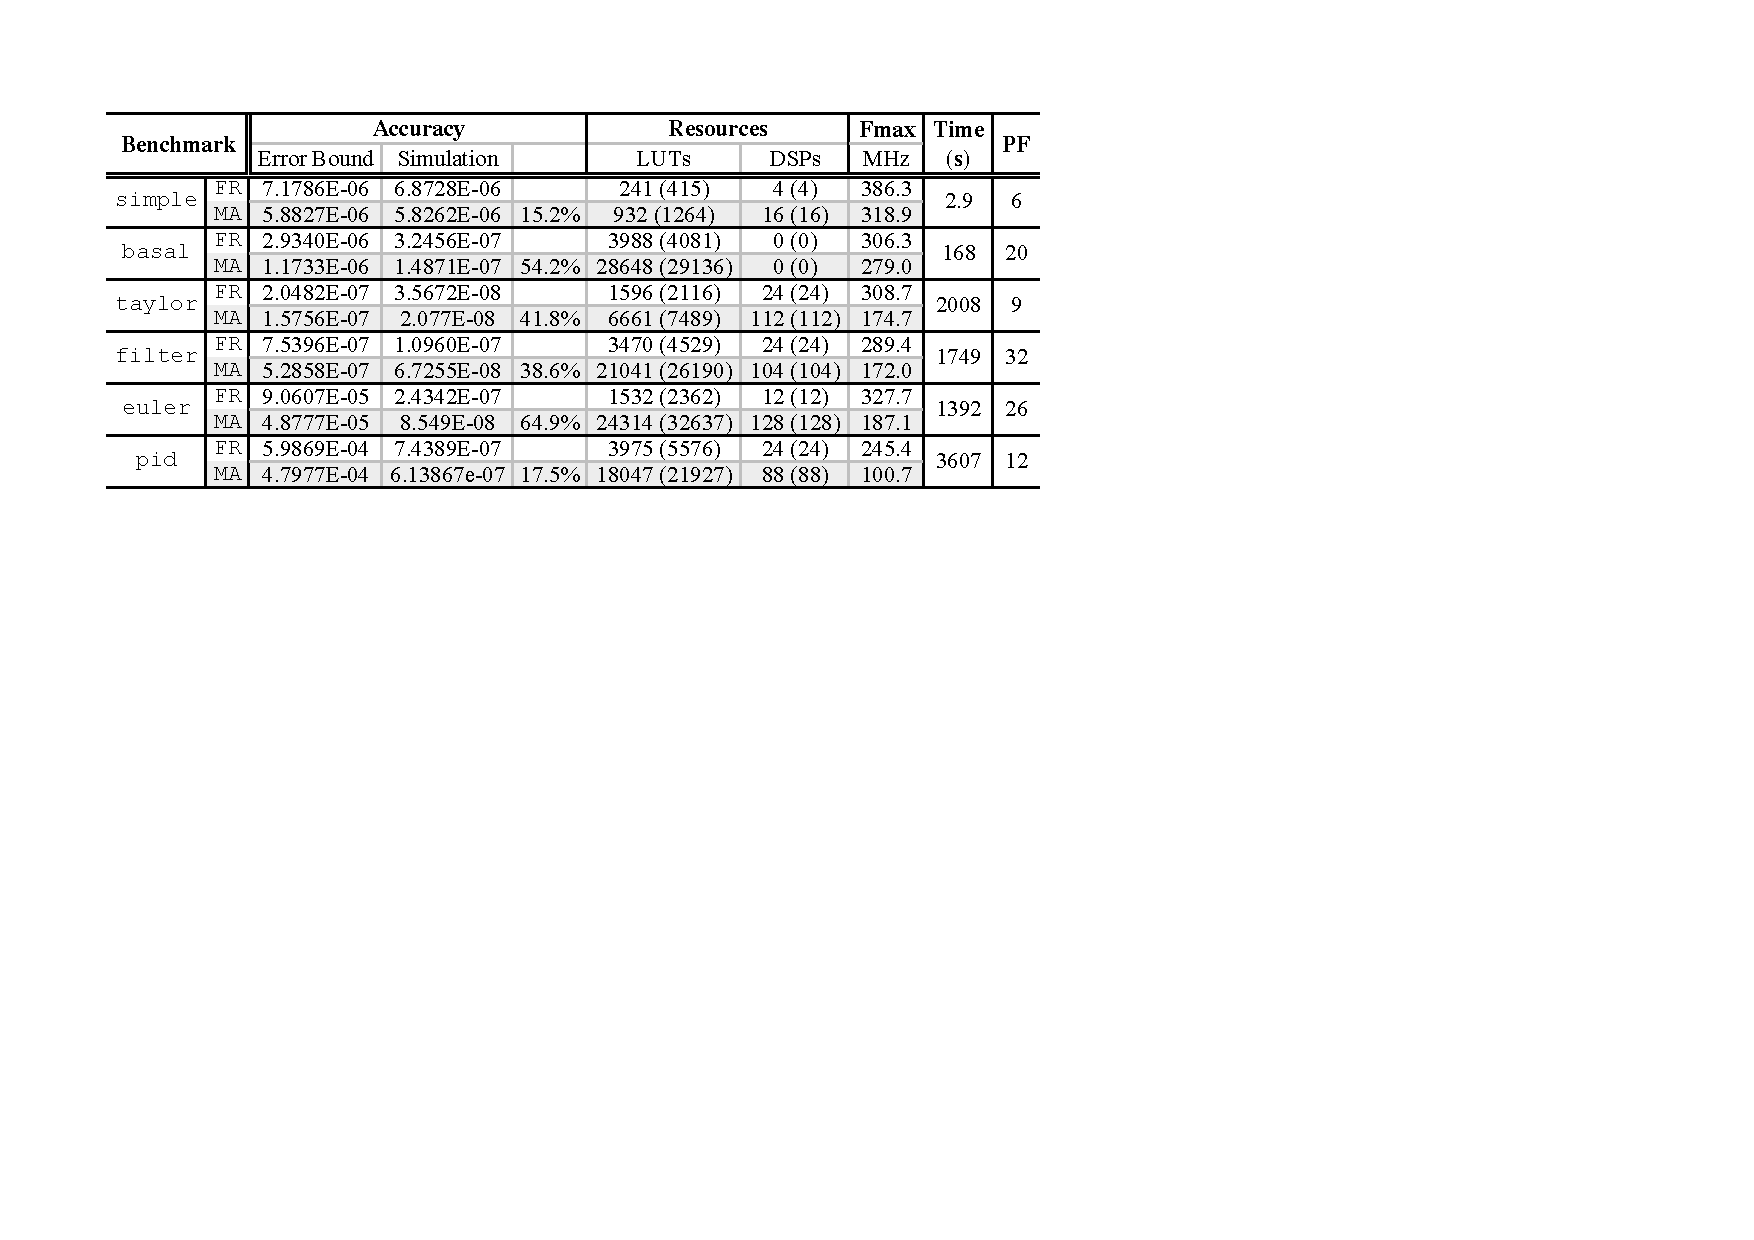
\includegraphics[width=\linewidth]{results}
    \captionof{figure}{%
    Table of optimization results.}\label{fig:results}
\end{figure}
\begin{figure}[ht]
    \centering
    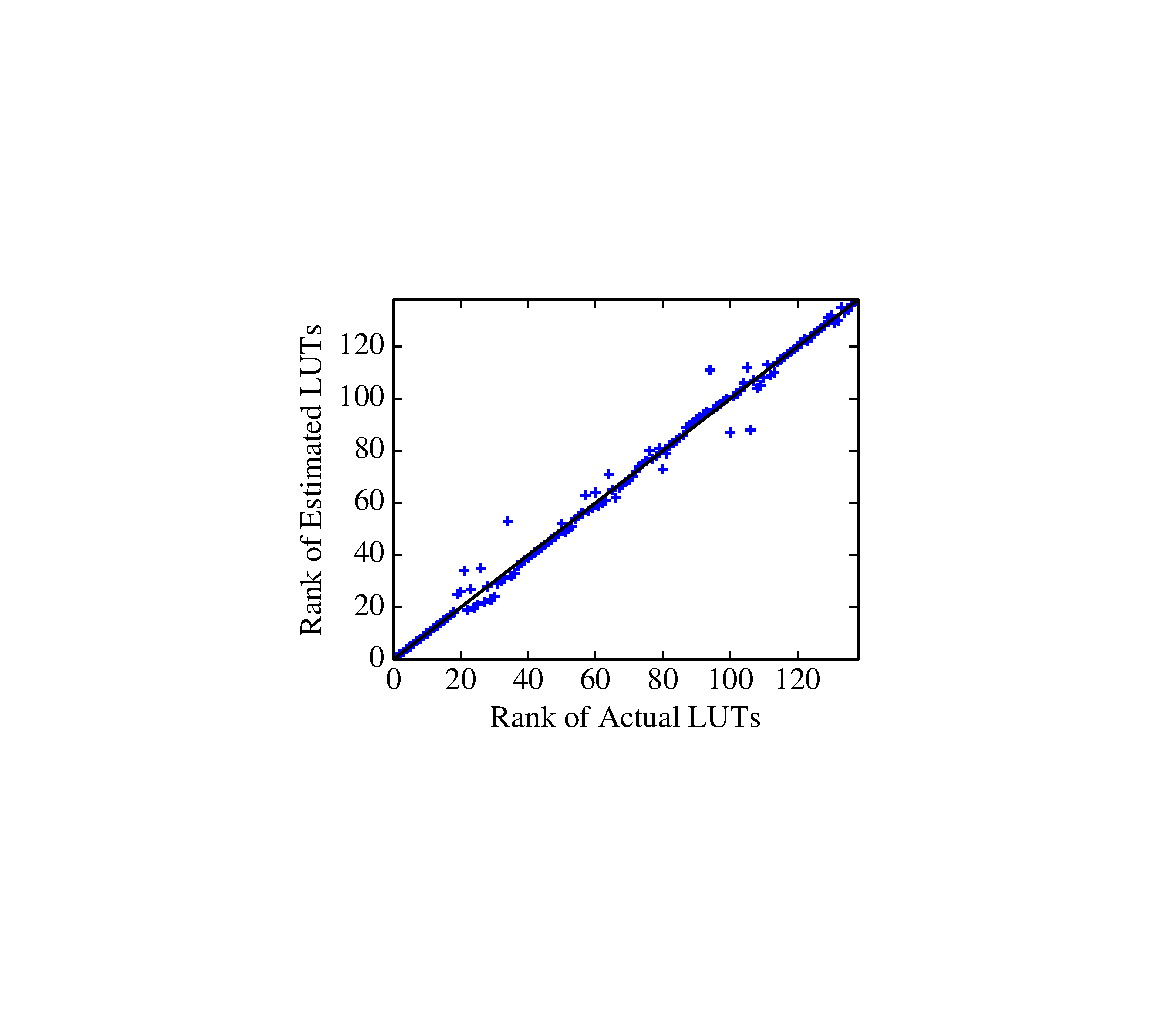
\includegraphics[scale=0.7]{rank}
    \captionof{figure}{%
    \mbox{The quality of resource estimation.}}\label{fig:rank}
\end{figure}

\begin{figure*}[ht]
    \centering
    \begin{minipage}{0.6\textwidth}
    \end{minipage}\quad\begin{minipage}{0.35\textwidth}
    \end{minipage}
\end{figure*}

The ``Resources'' columns show our estimation of the number of LUTs and
DSPs required for each of these programs, and the numbers in brackets are
the corresponding statistics obtained from Quartus synthesis.  Because
implementations on the Pareto frontier is only sensitive to how their LUTs
compare against each other, \ie~the rank, the Pareto frontier will not be
affected unless the rank is changed.  To ensure that the resource estimation
method used in our optimization can identify accurately whether an actual
implementations is on the Pareto frontier, we gathered 150 implementations
discovered across the benchmark examples, and for each one we rank its
number of estimated LUTs among them, and do the same for actual LUTs.
Figure~\ref{fig:rank} plots the rank of estimated LUTs against the rank of
actual LUTs, which shows the Pareto frontier we produced is very close to using
Quartus to count resources.

Because our benchmark examples are designed to be resource efficient, there
is no room for resource usage optimization of the original program.  However
we are able to consistently reduce the resource usage of a plain partial
loop unrolling by more than 25\%, because our optimization can discover
subexpression sharing opportunities, propagate constants values, and also
aggressively reduce the size of expressions by powerful reduction rules such as
$a - a = 0$ and $0 \times a = 0$.

Besides the choices of implementations that are either most accurate or most
resource efficient, each optimization also offers a wide selection of optimized
programs on the Pareto frontier.  For instance, Figure~\ref{fig:euler} shows
the Pareto frontier of \texttt{euler}, which has 26 different trade-off
options.  Furthermore, in the optimization of \texttt{euler}, our optimization
not only identifies that it is resource efficient when the two return variables
are computed by the same loop, but also by individually optimizing the
accuracy of the two variables, we produce a program with two loops, each with
a different goal, that is to compute their respective return variables as
accurately as possible, this generated a program that consists of two loops
that have completely different structures.  With this, we further widen the
trade-off curve with the most accurate option improving the accuracy by 65\%.
In Figure~\ref{fig:filter}, because the loop kernel of \texttt{filter} has the
expression $\sum_{i=0}^2{(a_i y_i + b_i x_i)}$, which has a large number of
equivalent expressions, without increasing the resource usage, our optimization
improves its accuracy by 14.5\%.  Because our Pareto frontier has three
dimensions, which are respectively accuracy, LUT utilization and the number of
DSPs, points within the shaded region optimize DSP count.

\begin{figure}[ht]
    \centering
    \subfloat[\texttt{euler}]{%
        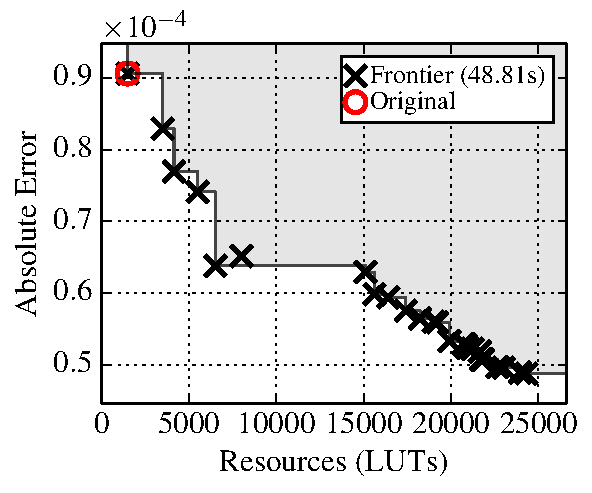
\includegraphics[width=0.6\linewidth]{euler}
        {}\label{fig:euler}
    } \\
    \subfloat[\texttt{filter}]{%
        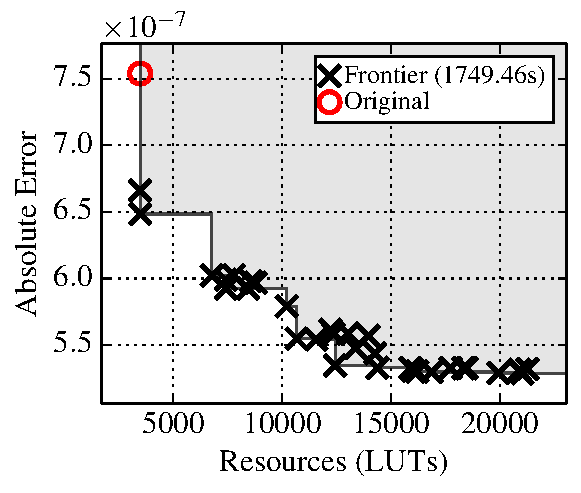
\includegraphics[width=0.6\linewidth]{filter}
        {}\label{fig:filter}
    }
    \caption{The Pareto frontier.}
\end{figure}

\section{Summary}
\label{so:sec:conclusion}

We provide a formal approach to the optimization of arithmetic expressions
for both accuracy and resource usage in high-level synthesis.  The method
proposed in this chapter and the associated tool, \soap, encompass three kind
of semantics that describe the accumulated roundoff errors, count operators in
expressions considering common subexpression elimination, and derive equivalent
expressions.  For a set of input expressions, the proposed approach works out
the respective sets of equivalent expressions in a hierarchical bottom-up
fashion, with a windowing depth limit and Pareto selection to help reduce the
complexity of equivalent expression discovery.  Using \soap, we improve either
the accuracy of our sample expressions or the resource utilization by up to
60\%, over the originals under single precision. \soap~enables a high-level
synthesis tool to optimize the structure as well as the precision of arithmetic
expressions, then to automatically choose an implementation that satisfies
accuracy and resource usage constraints.

Because we underpin our approach in formal semantics, it provides the
necessary foundation which permits us to extend the method for general
numerical program transformation in high-level synthesis.  Therefore in
Chapter~\ref{chp:progopt}, we base ourselves on the methodologies developed
in this chapter, and propose a structural approach to program optimization by
safely rewriting equivalent structures in numerical programs.


\chapter{Numerical Program Optimization}
\label{chp:progopt}

\chapter{Latency}


\chapter{Conclusion}

\chapter{Future Work}

We believe that it is possible to extend our tool for the multi-objective
optimization of arithmetic expressions in the following ways. First, Secondly,
it would be useful to further allow transformations of expressions while
allowing different mantissa widths in the subexpressions, this further
increases the number options in the Pareto frontier, as well as leads to more
optimized expressions. Thirdly, as an alternative for interval analysis, we
could employ more sophisticated abstract domains that capture the correlations
between variables, and produce tighter bounds for results. Finally, there
could be a lot of interest in the HLS community on how our tool can be
incorporated with Martin Langhammer's work on fused floating-point datapath
synthesis~\cite{langhammer}.


\cleardoublepage


% Back matter
{%
\setstretch{1.1}
\renewcommand{\bibfont}{\normalfont\small}
\setlength{\biblabelsep}{0pt}
\setlength{\bibitemsep}{0.5\baselineskip plus 0.5\baselineskip}
\printbibliography[nottype=online]
\printbibliography[heading=subbibliography,title={Webseiten},type=online,prefixnumbers={@}]
}
\cleardoublepage

\listoffigures
\cleardoublepage

\listoftables
\cleardoublepage

% \input{colophon}
% \cleardoublepage

% \input{declaration}
% \clearpage
% \newpage
% \mbox{}

\end{document}
